\chapter{Predizione della struttura di proteine (PSP)}

Il protein folding problem ha sia guidato che tratto beneficio dagli avanzamenti nei metodi sperimentali e computazionali\supercite{dill2008protein}. Uno dei maggiori obiettivi della biologia computazionale è proprio il PSP (Protein Structure Prediction), ovvero la predizione della struttura nativa tridimensionale di una proteina a partire dalla sua sequenza amminoacidica. Il PSP è il problema opposto al \textit{protein design} (la progettazione di nuove sequenze proteiche che abbiano delle specifiche attività).

\par Grazie al CASP, alla crescita del PDB e ai metodi per omologia veloce e di allineamento di sequenze i metodi computazionali hanno registrato notevoli progressi, come dimostra il livello raggiunto da AlphaFold. 

\par La predizione della struttura di proteine è uno strumento fondamentale in medicina per la comprensione delle malattie da misfolding, nell'industria farmaceutica per risparmiare anni di laboriosi e costosi esperimenti correntemente richiesti per lo sviluppo di un singolo farmaco (\textit{drug design}), in biotecnologia per il design di nuovi enzimi e in generale per acquisire maggior conoscenza sul protein folding in tutti i suoi lati.

\par La determinazione sperimentale della struttura delle proteine, discussa sotto, ha vissuto dei progressi significativi col passare degli anni ed è di grande importanza per i metodi computazionali di PSP.

\section{Determinazione sperimentale}

I biochimici conoscono oggi la sequenza amminoacidica per più di 225 milioni di proteine\supercite{proteienDBentries} (UniProt), con circa 4.5-5 milioni aggiunte ogni mese. La struttura tridimensionale è conosciuta per quasi 200.000 proteine\supercite{proteienDBentries} (PDB)\footnote{al 25 Gennaio 2022 sono presenti 197.514 strutture di macromolecole quindi non solo proteine ma anche acidi nucleici e altre strutture complesse\supercite{pdbStats}} con più di 10.000 strutture aggiunte ogni anno. 

- come le proteine sono studiate [alberts, 4.4 p.158]
- metodi sperimentali 
alberts p.168
pal 6 p.126 ma è molto tecnico
wiki-protein folding, 
baxevanis 12 p.363

• storia dei metodi sperimentali (Pal) \\
• cristallografia a raggi-x \\
• NMR, risonanza magnetica nucleare \\
• Cryo-EM (electron microscopy) \\
\subsection{Predizione guidata sperimentalmente}
kessel 3.5
pal 6.2.5 p.138

Anche quando gli scienziati hanno una proteina correttamente ripiegata fra le mani non è così semplice determinarne la sua esatta conformazione tridimensionale, considerando che si parla di strutture di migliaia di atomi.

\section{Strumenti informatici}
La piccola percentuale di strutture determinate e il gap che continua a crescere con le sequenze conosciute è una conseguenza della lentezza dei metodi sperimentali (e in parte dei progressi delle tecnologie di sequenziamento). I metodi computazionali, significativamente più veloci ed economici, potrebbero risolvere (almeno parzialmente) questo problema.

\subsection{Rappresentazione informazioni}
pal 6.4.1 p.145
Gu 10-13 p.468
baxevanis 12 p.367

\subsection{Database}
baxevanis 12 p.373, 1

\subsection{Visualizzazione proteine}
pal 6.4 p.146, ottima
kessel p.174 (2.3 GRAPHIC REPRESENTATIONS OF PROTEINS)
\subsection{CASP}

\section{Workflow PSP, input, output, metriche}
- paper Soft computing
\subsection{Proprietà dei dati di input}
\subsection{Allineamento di sequenze}
- protein sequence alignment (poi MSA)
[Burkowski 6 p.167]
baxevanis 8 p.227


\subsection{Output: modelli, ... [..]}
\subsection{Metriche di valutazione}
- Gu 16 p.655 GENERAL APPROACH TO STRUCTURE COMPARISON AND ALIGNMENT
baxevanis 12 p.386

\section{Paradigmi per approssimazione biologica}
kessel 3.4 [computational methods for structure prediction]
pal 15.3.2 Computational structure prediction. Molto breve
pal 18.1 [molecular dynamics]
psp-wiki [abbastanza discorsivo]
prot-eng-wiki[molto breve]
Gu 28-33 [serie di articoli messi insieme, sembra stra interessante]
baxevanis 12 p.385 \\ \\


I numerosi metodi computazionali per il PSP possono essere raggruppati in due categorie di approcci\footnote{La presente sezione sui paradigmi per approssimazione biologica segue e si basa sul capitolo 3.4 di \fullcite{kessel_ben-tal_2018}}:
\begin{itemize}
	\item \textit{ab initio} (o \textit{de novo}), approccio fisico, nei quali la struttura è predetta da zero usando principi fisici
	\item \textit{template-based}, dove vengono usate informazioni da strutture 3D note di proteine. Questo approccio è ulteriormente divisibile in:
	\begin{itemize}
		\item \textit{homology modeling}, basato su confronti sequenza-sequenza tra la proteina da predire e il modello
	\item \textit{fold recognition}, basato su altre similitudini fra modello e proteina da predire
	\end{itemize}
\end{itemize}

\subsection{Ab initio}
Il metodo più lineare e a prima vista ovvio per predire la struttura nativa di proteine è seguire la natura, simulando accuratamente come le forze fisiche guidino la proteina a ripiegarsi e usare questa simulazione per riprodurre il processo di ripiegamento su proteine con strutture sconosciute. \textit{Ab initio}, termine latino, significa infatti "dall'inizio".

\par Il primo problema che sorge è superare il paradosso di Levinthal. Per farlo si assume un profilo energetico a imbuto del ripiegamento, ovvero la premessa termodinamica che la forma nativa di una proteina sia lo stato in cui risulta avere più bassa energia libera, o più precisamente (richiamando la definizione di struttura nativa data nella sez. \ref{sec:energetica}) quella conformazione avente minore energia libera tale da mantenere il livello di dinamicità richiesto alla proteina per svolgere la sua funzione biologica.

\par Le predizioni nell'approccio \textit{ab initio} sono pertanto \textit{energy-based}. In quanto tali usano solo informazioni sul tipo di atomi nel sistema, le loro posizioni relative nello spazio tridimensionale e le loro interazioni con gli altri atomi. Viene poi calcolato l'intero contenuto di energia del sistema e le forze agenti su ogni atomo. L'energia totale di un sistema (\textit{free energy}) può essere decomposta in varie componenti: cinetica, potenziale, termica, ecc. . È l'energia libera che determina la stabilità del sistema.

\par Sebbene vi siano differenti metodi in questo approccio, tutti condividono due caratteristiche di base:
\begin{itemize}
	\item calcolano il contenuto di energia del sistema in una singola configurazione
	\item campionano numerose configurazioni e ne trovano una con la minor energia libera
\end{itemize}

Per \textit{configurazione} si intende la disposizione complessiva di tutti gli atomi di tutti i componenti del sistema (proteina, solvente, ioni, membrana, ecc.) mentre la posizione collettiva dei soli atomi della proteina viene chiamata \textit{conformazione}.

\par Per descrivere in maniera affidabile tutte le forze fisiche operanti sul sistema tra i differenti atomi bisognerebbe descriverne la distribuzione di tutti gli elettroni, il che richiede però calcoli di meccanica quantistica (QM). Le forze, in un sistema molecolare, risultano dalla distribuzione spaziale degli elettroni attorno agli atomi. Sfortunatamente questi calcoli sono computazionalmente molto costosi e una rigorosa caratterizzazione di un sistema macromolecolare, con milioni di atomi, è al momento insostenibile. Calcoli di QM su una singola conformazione di una piccola proteina possono richiedere mesi, tempi troppo lunghi se si ha l'obiettivo di provare tante configurazioni per sceglierne una finale. 

\subsubsection{Molecular mechanics}

\par Per le ragioni sopra elencate gli scienziati spesso investigano sistemi macromolecolari usando approssimazioni delle reali forze in essi. Il campo da cui i calcoli per le approssimazioni sono presi è chiamato \textit{molecular mechanics} (MM), poiché approssima sistemi molecolari usando espressioni prese dalla meccanica newtoniana classica:
\begin{itemize}
	\item le descrizioni che richiederebbero calcoli di QM vengono ignorate
	\item le rappresentazioni sono \textit{esplicite}: prendono in considerazione tutti gli atomi (vedi fig. \ref{fig:descrizione-esplicita-mm})
	\item il contenuto di energia è descritto usando un \textit{campo di forza} nel quale gli atomi e i legami covalenti sono trattati come palline e molle
\end{itemize}

Il campo di forza sopra accennato descrive l'energia potenziale del sistema. Da notare che l'energia potenziale (intesa come entalpia) è solo una delle due componenti dell'energia libera, l'altra è l'entropia, vedi sez. \ref{sec:energetica}).

Il campo di forza è un'energia di posizione: l'energia di un oggetto in una specifica posizione all'interno di un campo (gravitazionale, elettrico, magnetico, ecc.). Nelle molecole l'energia potenziale è la somma di tutti gli effetti dei campi elettrici atomici\footnote{gli atomi possiedono, in base alla loro eventuale carica, campi elettrici che influenzano gli altri atomi} in una determinata posizione. Si può approssimare l'energia potenziale all'energia risultante da tutti i legami covalenti e le interazioni non covalenti, escluse quelle non polari \footnote{un esempio di interazione non polare è l'effetto idrofobico. Vengono escluse poiché coinvolgono principalmente cambiamenti di entropia nel solvente}, in una singola configurazione del sistema.

\begin{figure}[!htb]
	\centering
	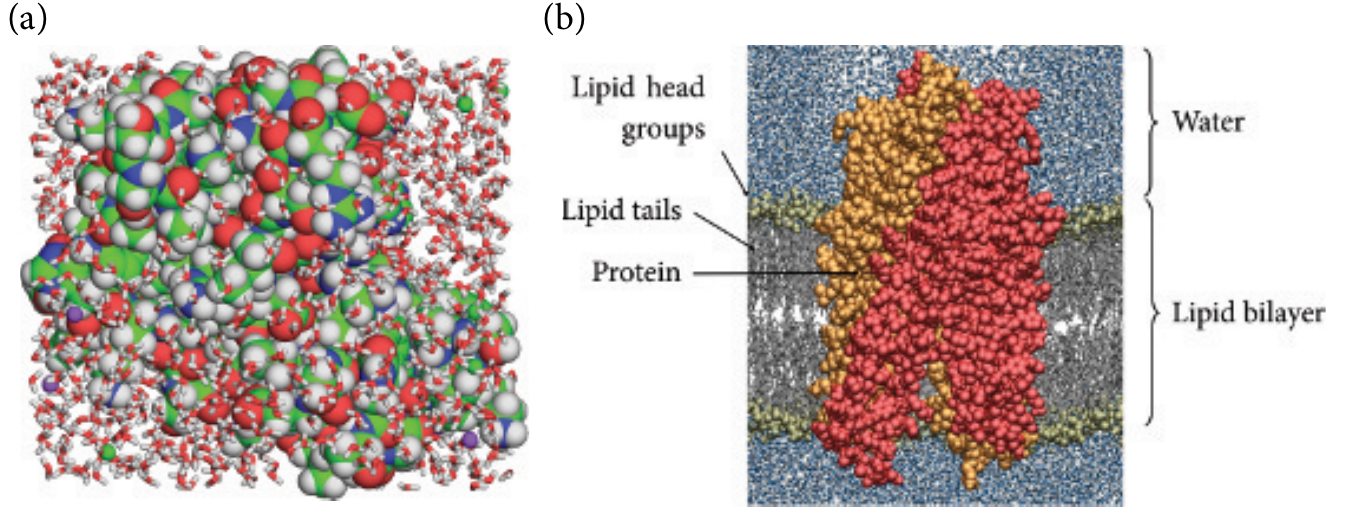
\includegraphics[scale=0.4]{images/esplicita-mm.png}
	\caption{Descrizioni esplicite nei calcoli di MM. (A) una piccola proteina immersa in un solvente composto da molecole d'acqua e ioni (Na$^{+}$, Cl$^{-}$). La proteina è rappresentata come sfere di atomi, l'acqua come bastoncini e gli ioni come piccole sfere magenta e gialle. (B) una proteina trasportatrice in un doppio strato lipidico, circondato da ambiente acquoso. La proteina e le teste dei lipidi sono rappresentate in modo space-fill, mentre l'acqua e le code dei lipidi con rappresentazione wire-frame. Fonte \cite{kessel_ben-tal_2018}}
	\label{fig:descrizione-esplicita-mm}
\end{figure}

\par La descrizione approssimata fornita dal campo di forza permette di calcolare l'energia potenziale di molti sistemi macromolecolari in meno di un secondo. \\

\par Una variante del MM è la \textit{QM/MM} nella quale i calcoli di QM sono indirizzati solamente su una piccola parte della proteina che contiene residui funzionali importanti. Le altre regioni sono soggette invece a MM, con calcoli molto più veloci. Questo approccio è stato introdotto da Warshel, Levitt e Karplus.

\subsubsection{Spazio configurazionale}

\par Assumendo l'accuratezza del campo di forza, il calcolo dell'energia potenziale di un sistema consente di determinare la stabilità di una configurazione. L'idea iniziale potrebbe essere quella di considerare tutte le possibili locazioni atomiche del sistema, calcolare l'energia potenziale in ogni caso e scegliere quella con la minor energia. Come si può facilmente intuire ciò risulta essere un procedimento troppo oneroso, in quanto si devono considerare anche gli atomi del solvente (ed eventuali ligandi o cofattori). Anche solo il numero delle possibili configurazioni atomiche è difficile da calcolare.

\par Per superare questo problema vengono usati metodi per ridurre lo spazio di ricerca nello spazio configurazionale. Ci sono vari metodi di ricerca nello spazio configurazionale, ad esempio: \textit{systematic search }(grid search basata su dettagli geometrici), \textit{model-building model }(usa frammenti molecolari), \textit{random approach }(movimenti random sul piano cartesiano da una configurazione iniziale), \textit{distance geometry} (usa una matrice di distanze atomiche), \textit{Monte Carlo method} (modifiche random e accettazione probabilistica di configurazioni a livelli energetici maggiori)\supercite{ROY2015151}.

\par Il metodo più semplice è chiamato \textit{energy minimization}:

\begin{enumerate}
	\item si parte da una configurazione arbitraria
	\item si calcola l'energia potenziale. Viene derivato questo valore su differenti posizioni nel sistema in modo da calcolare le forze agenti su ogni atomo dalla rimanente parte del sistema
	\item un piccolo cambiamento è introdotto nella posizione di ogni atomo, in risposta alle forze applicate su ognuno di essi dal resto del sistema (in accordo a quanto calcolato nel precedente step)
	\item se la nuova configurazione ha un'energia minore viene adottata
	\item altrimenti questa viene scartata e viene creata una nuova configurazione
	\item si ritorna allo step 3 finché non si trovano più configurazioni con minor energia
\end{enumerate}

Il metodo passa da una configurazione all'altra scendendo con il gradiente della superficie dell'energia potenziale finché non converge in un \textit{punto di minimo locale}. Tutte le procedure di \textit{energy minimization }tendono a rimanere bloccate in un minimo locale di energia non riuscendo spesso a raggiungere il minimo globale a causa di \textit{barriere energetiche} da scavalcare per raggiungere una configurazione con energia minore (vedi fig. \ref{fig:energy-minimization} e \ref{fig:imbuto}).

\begin{figure}[!htb]
	\centering
	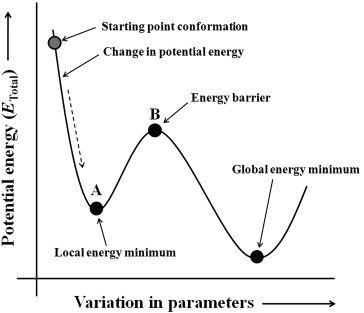
\includegraphics[scale=1]{images/energy-minimzation.jpg}
	\caption{Differenti fasi energetiche di una molecola durante la sua minimizzazione energetica. Fonte\cite{ROY2015151}}
	\label{fig:energy-minimization}
\end{figure}

\subsubsection{Molecular dynamics}

È possibile spingere l'algoritmo di minimizzazione energetica fuori da punti di minimo locale fornendo energia extra, ad esempio innalzando la temperatura del sistema (ovvero aggiungendo calore virtuale). L'energia aggiunta consente agli atomi del sistema di incrementare i loro movimenti e nuove configurazioni fuori dalle barriere energetiche vengono create. Questo metodo è chiamato \textit{Molecular dynamics }(MD) e si focalizza sui movimenti dipendenti dal tempo degli atomi nel sistema. I calcoli sono realizzati in accordo alla meccanica classica. 

\par Agli atomi viene assegnata una veloctià iniziale (proporzionale alla temperatura) e continuano a muoversi nello spazio secondo i corrispondenti cambiamenti nell'energia potenziale del sistema. Il movimento di ogni atomo nel sistema è calcolato in base alla sua energia in quel dato momento.

\par Le similuazione di MD sono eseguite in cicli ripetitivi di \textit{riscaldamento} e \textit{raffreddamento} (metodo conosciuto nel mondo informatico come \textit{simulated annealing}, in riferimento al processo di tempra dei metalli). Nella fase di riscaldamento vengono superate le barriere energetiche mentre la fase di raffreddamento (seguita dall'\textit{energy minimization}) consente al sistema di rilassarsi in configurazioni con minor energia.

\par Un metodo comune per rendere la ricerca con MD più efficiente è di spezzarla in due fasi:
\begin{itemize}
	\item ricerca a bassa risoluzione per trovare una collezione di strutture con interazioni non polari (basato sulla nozione che il nucleo delle proteine globulari sia idrofobico)
	\item ricerca ad alta risoluzione fra le strutture selezionate nel primo step
\end{itemize}

\subsubsection{Limiti dell'approccio fisico}
I metodi di MM/MD trovano difficilmente impiego in processi biologici rilevanti come il protein folding. Un problema risiede nell'approssimazione dell'energia libera con un campo di forza, il quale fornisce sì l'energia potenziale ma non l'entropia. L'unico modo per stimare l'entropia e l'energia libera dai calcoli per l'energia potenziale è eseguire questi calcoli su tutte le possibili configurazioni del sistema e poi integrarli. Il problema risiede proprio nelle rappresentazioni esplicite nelle simulazioni in MD.


\subsection{Homolgy}
\subsection{Threading}
\subsection{Metodi integrativi [..]}
\subsection{applicazioni specifiche [..]}
\subsubsection{Loop modeling}

- predictive methods
baxevanis 7

\section{Paradigmi nel soft computing}
\subsection{ANN, EC, SVM, .. [..]}
\subsection{altri approcci [..]}

\section{Storia della comprensione delle proteine}
- alberts p.160
- psp-wiki
- levitt 2001, birth of structural biology

\subsection{primi approcci}

L'approccio \textit{ab initio} è emerso negli anni '60 a partire dal campo della chimica computazionale. Nel 2013 il premio Nobel per la chimica è stato assegnato proprio a quegli scienziati che hanno contribuito sin da quegli anni al campo della biofisica molecolare computazionale (Warshel, Levitt, Karplus).

\par Le predizioni di strutture basate sui metodi \textit{ab initio} sono emerse nella metà degli anni '80, prima per piccoli peptidi e poi per polipeptidi. Il primo programma per calcolare l'energia potenziale nelle proteine è stato sviluppato nel 1969 da Lifson e Levitt\supercite{levitt1969refinement}.

\par La prima simulazione di MD su una proteina è stata realizzata nel 1977 da McCammon, Gelin e Karplus\supercite{mccammon1977dynamics}, studiando la dinamica di ripiegamento di una proteina di 58 amminoacidi rappresentata esplicitamente ma simulata nel vuoto. Questo studio seguì il lavoro pionieristico di Levitt e Warshel del 1975 (\textit{Computer simulation of protein folding}\supercite{levitt1975computer}) sulla stessa proteina che era però rappresentata in modo più semplicistico: ogni amminoacido era rappresentato da due sfere. 



\subsection{anni '90, database, omologia, progetto genoma}
\subsection{CASP e AlphaFold}

\clearpage